\section{Project Management with Scrum}

This section outlines the key aspects of project management with Scrum including the product backlog, use case diagram, sprint planning, and interface prototyping.

\subsection{Backlog Features}
\begin{longtable}{|c|p{0.8\textwidth}|}
	\hline
	\textbf{ID} & \textbf{User Story}                                                                                                                                            \\
	\hline
	\endhead
	1           & As a new user, I want to register for an account with a password, and email so that I can access the system.                                                   \\
	\hline
	2           & As a user, I want to log in to my account using my email and password so that I can securely access my information.                                            \\
	\hline
	3           & As a user, I want to reset my password using my email in case I forget it, to regain access to my account.                                                     \\
	\hline
	4           & As a user, I want to create a new organization with a unique name, becoming its administrator, so I can manage users and templates within that organization.   \\
	\hline
	5           & As a user, I want to view a list of all organizations I'm part of, so I can easily navigate and manage them.                                                   \\
	\hline
	6           & As a user, I want to have access to the shared work (templates, emails, media) within my organization, ensuring I can collaborate effectively.                 \\
	\hline
	7           & As an administrator of an organization, I want to deactivate or remove users from my organization, ensuring security and access control.                       \\
	\hline
	8           & As an administrator of an organization, I want to add other users to my organization and assign them specific roles , so I can control access and permissions. \\
	\hline
	9           & As an administrator of an organization, I want to view and manage the roles associated with each user, ensuring proper permissions are maintained.             \\
	\hline
	10          & As a user, I want to create a new email template, so I can use it for sending emails.                                                                          \\
	\hline
	11          & As a user, I want to edit and update my email templates, ensuring the information is current and accurate.                                                     \\
	\hline
	12          & As a user, I want to view a list of all my email templates, so I can quickly access and manage them.                                                           \\
	\hline
	13          & As a user, I want to search for specific email templates or medias within my organization, making it easier to locate relevant information.                    \\
	\hline
	14          & As a user, I want to create and manage email template drafts, allowing me to work on them before finalizing and sending.                                       \\
	\hline
	15          & As a user, I want to send an email using a selected template to a specified recipient, tracking the sent email's status and timestamp.                         \\
	\hline
	16          & As a user, I want to view a history of all the emails I have sent, including their status and timestamp, for reference.                                        \\
	\hline
	17          & As a user, I want to create and manage campaigns, allowing me to organize and track my marketing efforts.                                                      \\
	\hline
	18          & As a user, I want to have reports of my campaigns, so I can analyze their effectiveness and make informed decisions.                                           \\
	\hline
	\caption{Backlog Features}
	\label{tab:Backlog Features}
\end{longtable}


\newpage

\subsection{Global Use Case Diagram}
Figure 2.19 offer us a global overview by presenting a visual description of the functional
behaviour of our tool. This diagram sums up the interactions among the actors and the
diverse use cases within the system.

\begin{figure}[ht]
	\centering
	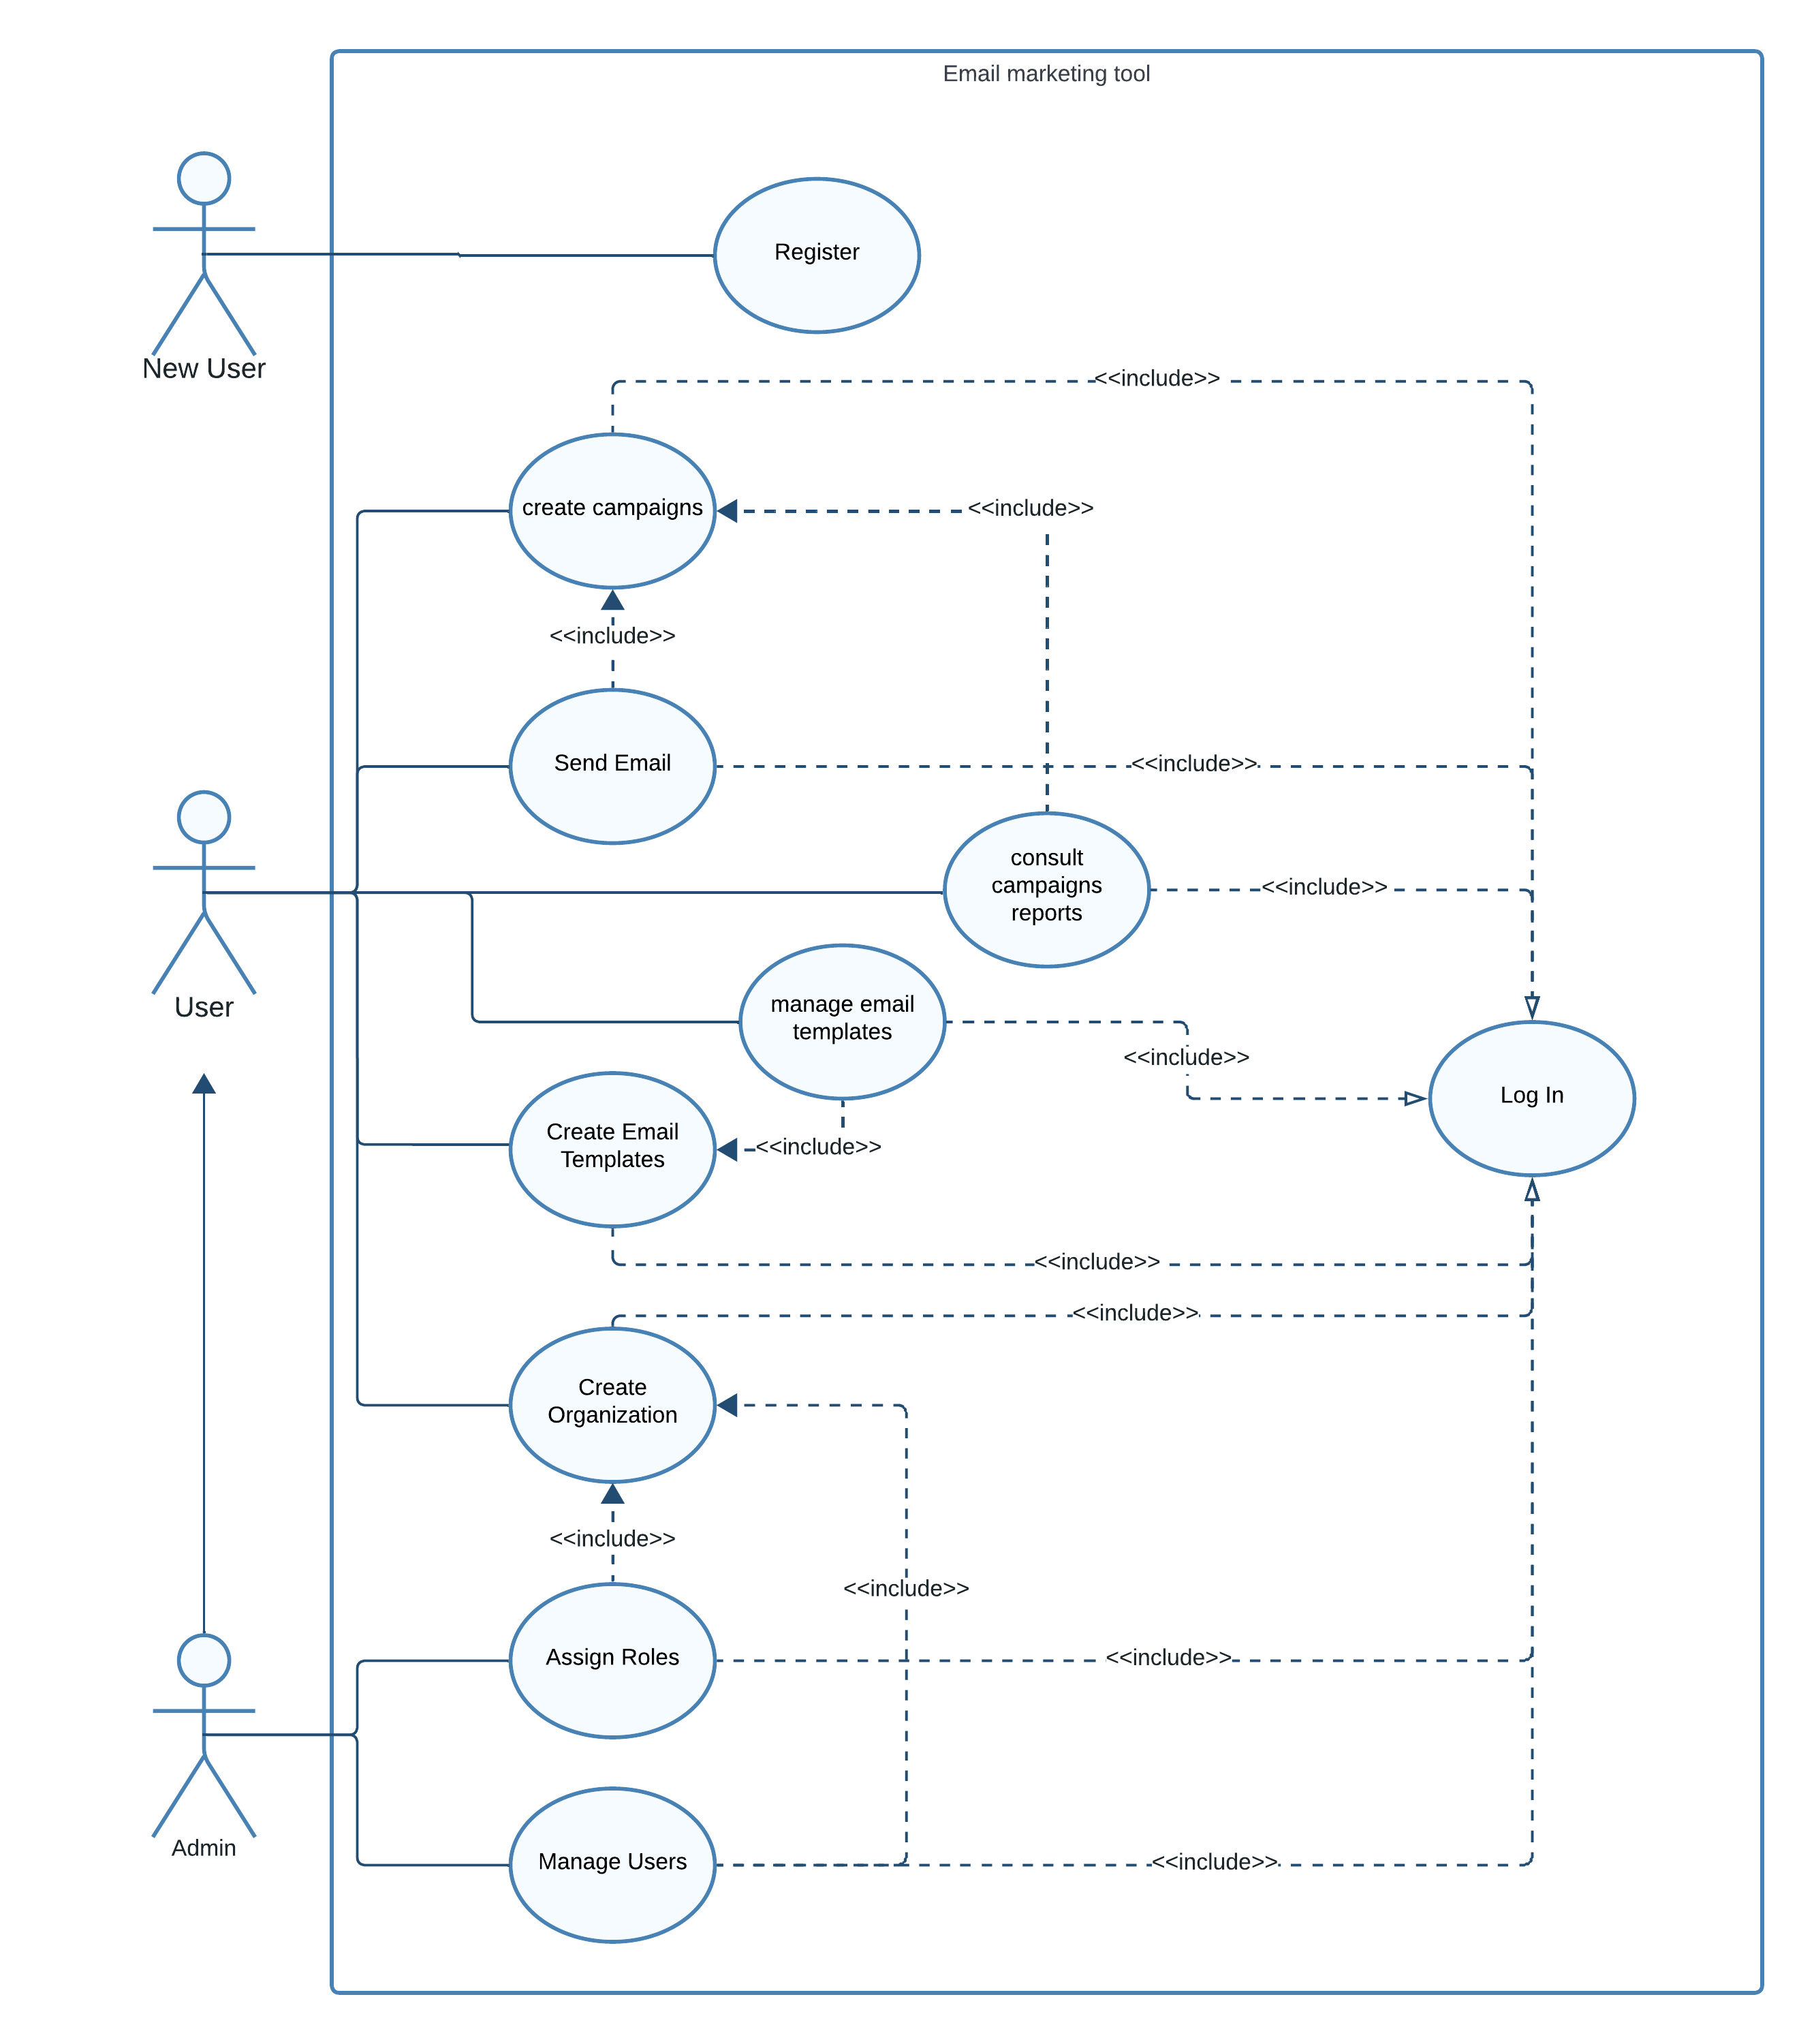
\includegraphics[width=\linewidth]{Images//images/global use case diag.png}
	\caption{Global Use Case Diagram}
	\label{fig:Global Use Case Diagram}
\end{figure}

\newpage

\subsection{Sprint Planning}

In Figure 2.20, we present the sprint planning for the project. Each sprint had a specific duration and goals.
The initial phase was dedicated to learning the necessary tools for the project.
The sprint 1 was dedicated to building the email builder and enabling email sending.
In the sprint 2, we implemented email tracking functionality and creating and managing campaigns.
The final sprint was spent on media and organization management, and conducting final testing and bug fixing across all features.
This structured approach allowed us to systematically tackle different aspects of the project, ensuring thorough development and testing of each feature.
As a result, all planned features were successfully implemented and thoroughly tested within the project timeline.

\begin{figure}[ht]
	\centering
	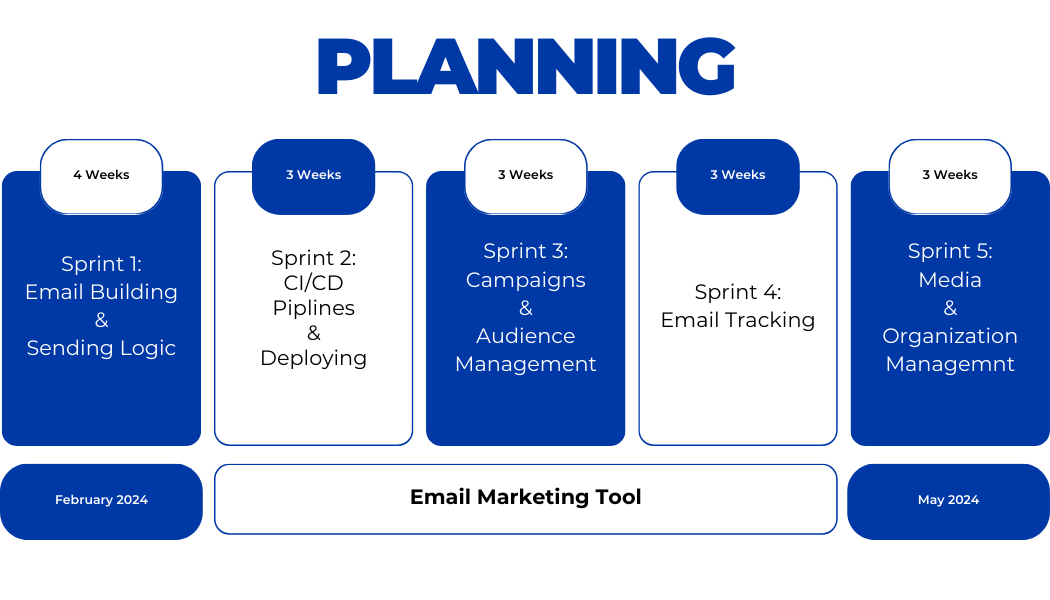
\includegraphics[width=\linewidth]{Images//images/planning.png}
	\caption{Sprint Planning}
	\label{fig:Sprint Planning}
\end{figure}
